\section{Zusammenfassung und Diskussion}
	Im Experiment wurde die mittlere Lebensdauer von Myonen mit Hilfe einer Koinzidenzmessung untersucht. Zur Abschätzung wurde das Maximum-Likelihood-Verfahren eingesetzt, wobei drei verschiedene Verteilungen zugrunde gelegt wurden: ein exponentielles Zerfallsgesetz, eine Poisson- und eine Normalverteilung. Tabelle \ref{tab:results} fasst die Ergebnisse für die Kanäle 20 bis 175 zusammen.
	\begin{table}[ht]
		\centering
		\begin{tabular}{c|c}
		Verteilung & mittlere Lebensdauer $\tau /\unit{\mu s}$\\
		\hline
		Exponentielles Zerfallsgesetz	&	$3,52 \pm 0,03$\\
		Poissonverteilung				&	$2,24 \pm 0,03$\\
		Normalverteilung 				&	$2,23 \pm 0,01$
		\end{tabular}
		\caption{Schätzwerte für die mittlere Lebensdauer der Myonen.}
		\label{tab:results}
	\end{table}
	Man beobachtet, dass die Ergebnisse für die Poisson- und die Normalverteilung sehr gut zum Literaturwert (\ref{eq:lit}) passen. Das exponentielle Zerfallsgesetz kommt nur mit einer anderen Kanalkonstellation an dieses Ergebnis heran, weshalb diese Methode nicht die optimale Wahl zur Schätzung dieses Parameters ist. Die Genauigkeit des Ergebnisses wird vor allem durch zufällige Koinzidenzen und den $\mu^-$-Einfang begrenzt, welche die enorm hohen Zählraten in den Kanälen geringer Lebensdauer erzeugen. Man könnte die Messung verbessern, indem man die Detektoren besser von der natürlich auftretenden Strahlung abschirmt. Zur exakteren Bestimmung der Lebensdauer könnte man Myonen durch Pion-Erzeugung an einem Teilchenbeschleuniger beobachten und vermessen.
	

\newpage
\section{Anhang}
\subsection{Messprotokoll}
In diesem Abschnitt befindet sich das handschriftlich erstellte Messprotokoll mitsamt der uns gegebenen Aufgabenstellung.\\
	\begin{figure}[ht]
					\centering
					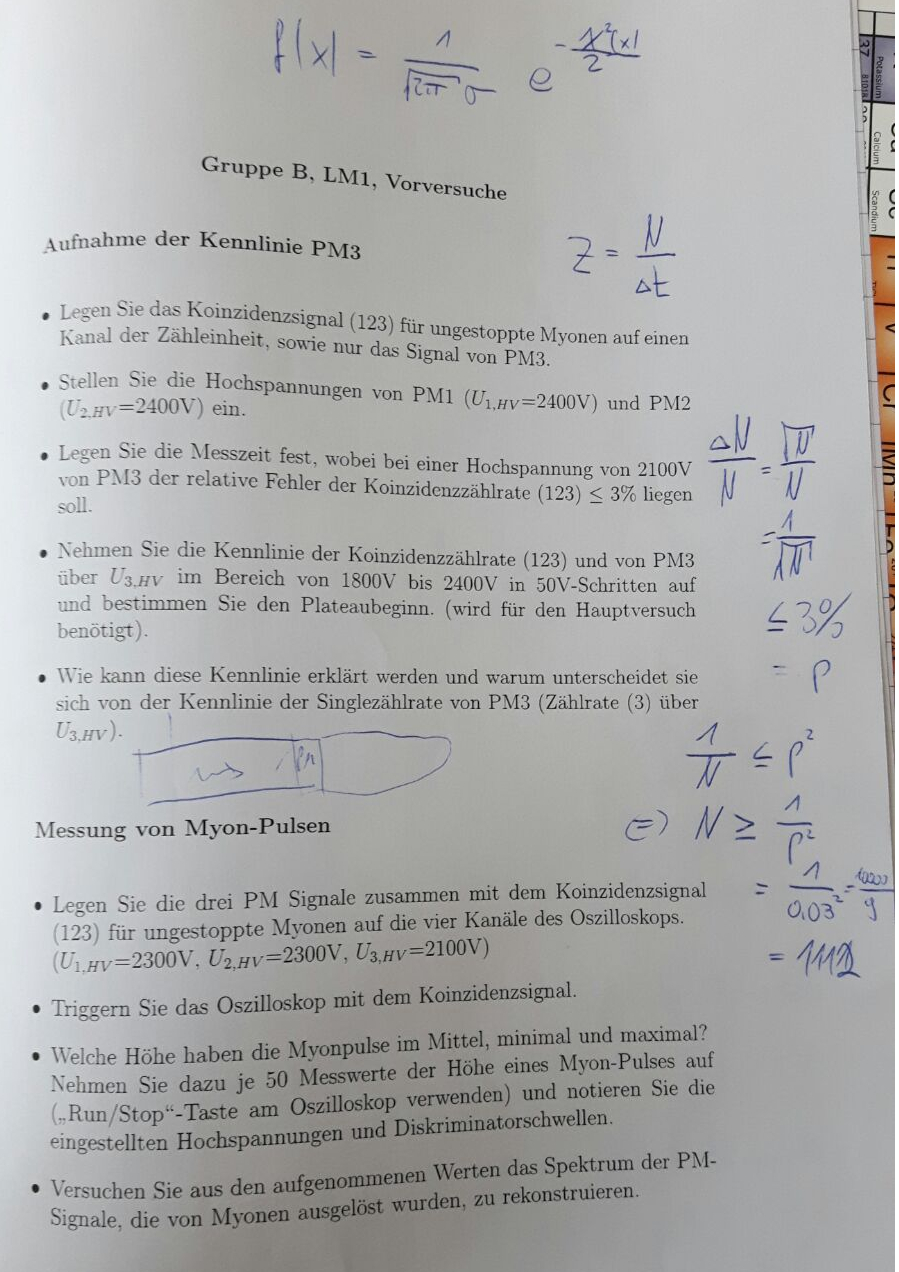
\includegraphics[width = 1.\linewidth]{pic/aufgabe.jpg}
					\caption{Aufgabenstellung}
	\end{figure}
	\begin{figure}[ht]
						\centering
						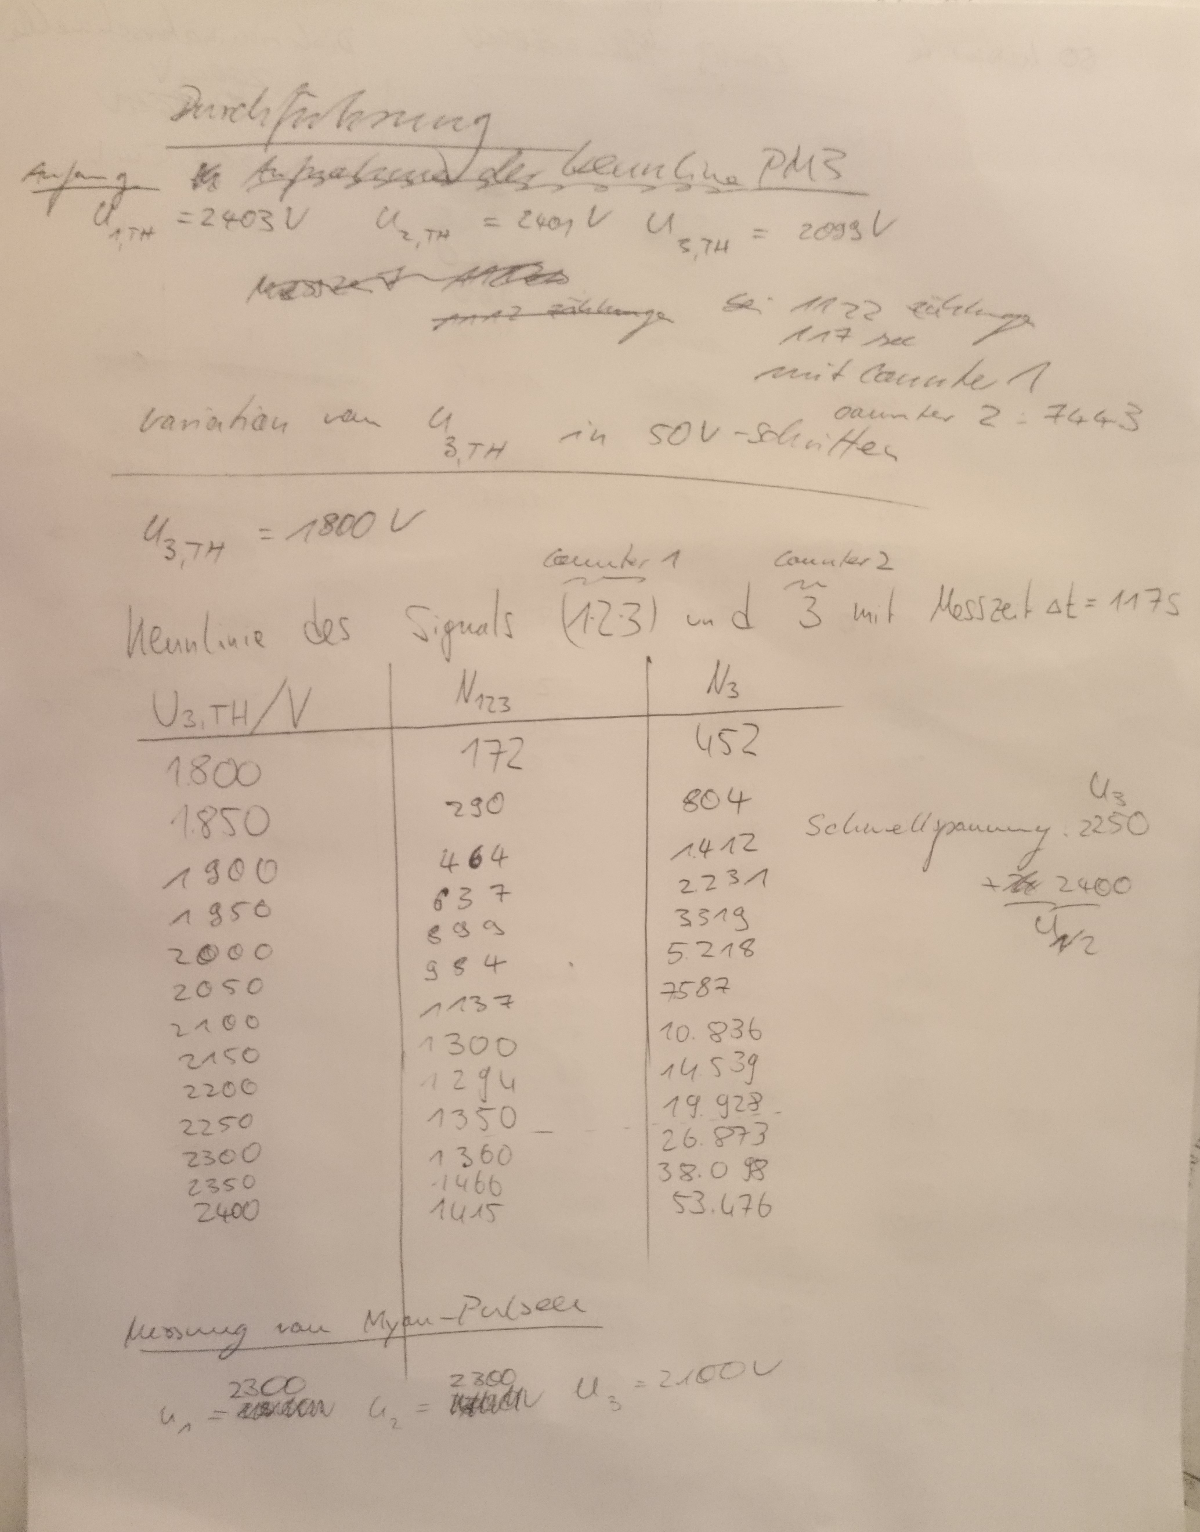
\includegraphics[width = 1.\linewidth]{pic/mess1.png}
						\caption{Messprotokoll Teil 1}
	\end{figure}
	\begin{figure}[ht]
						\centering
						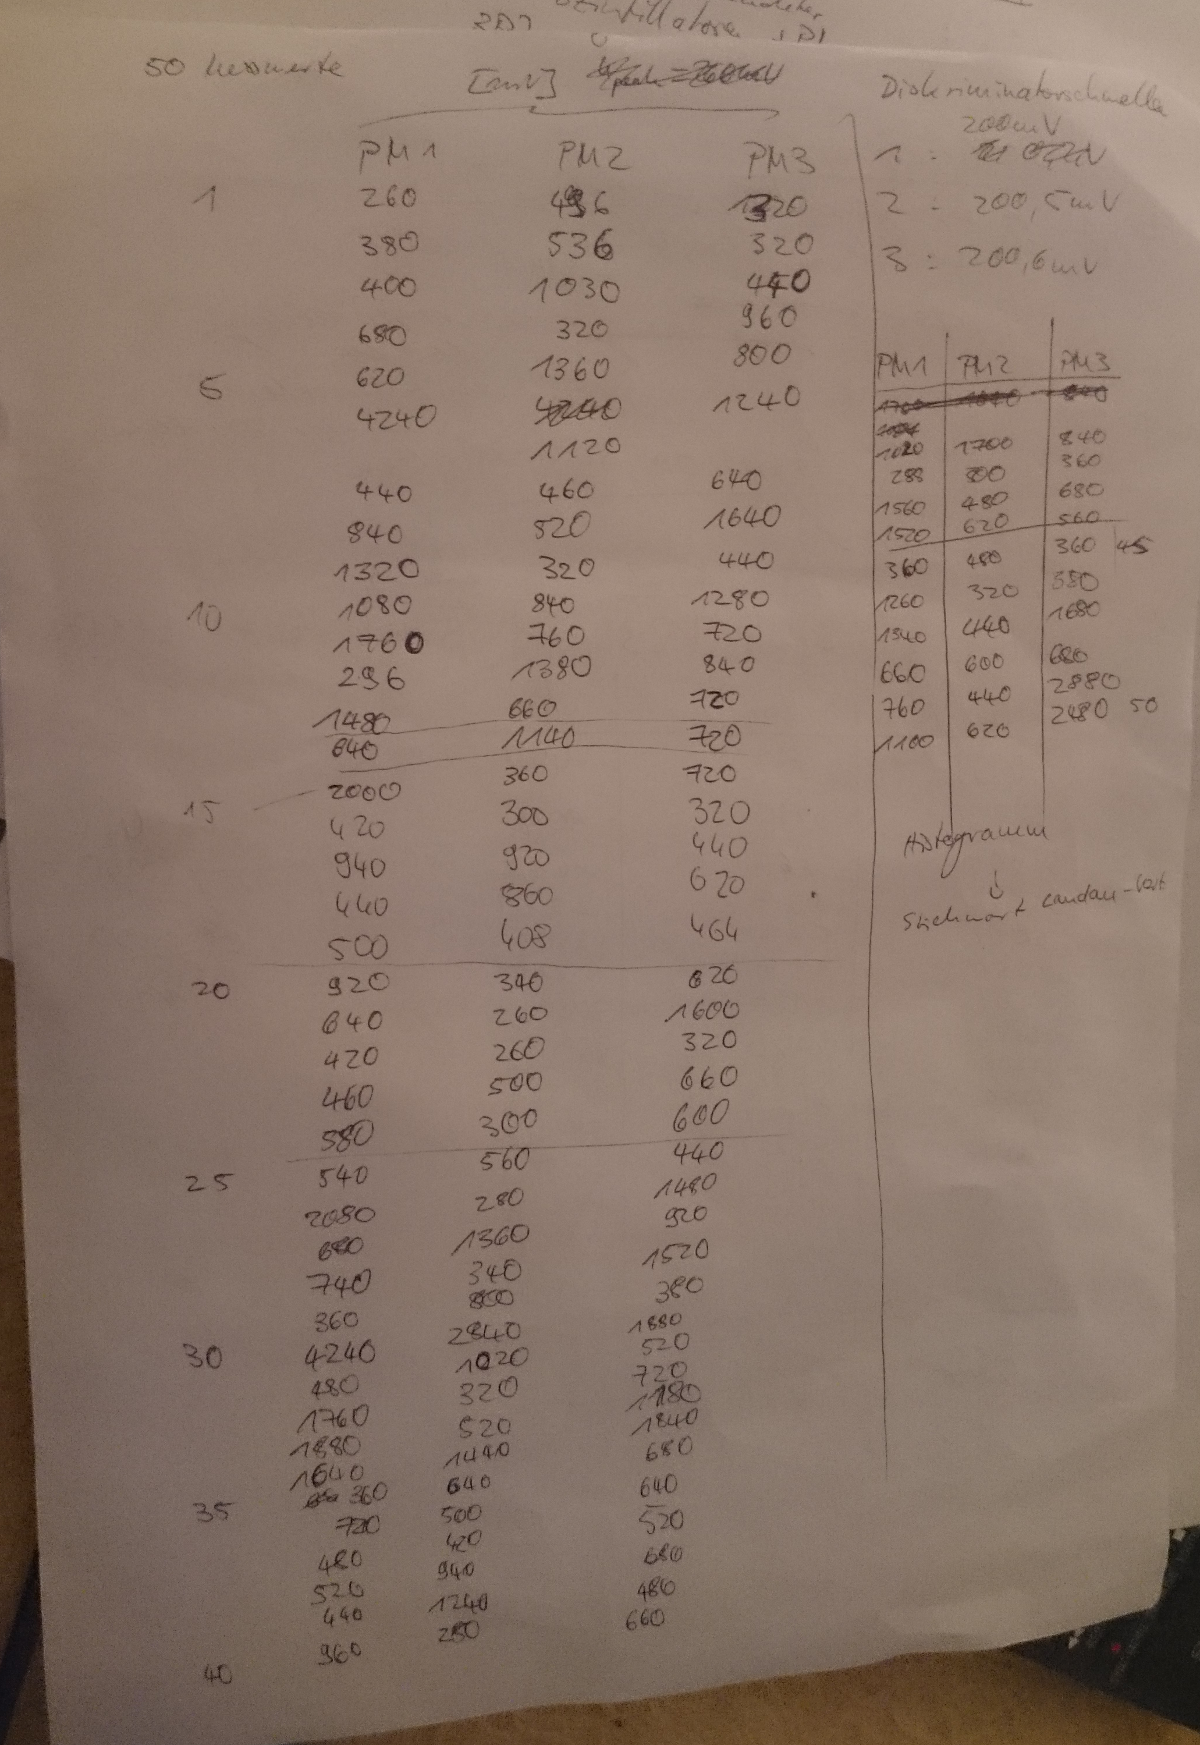
\includegraphics[width = 1.\linewidth]{pic/mess2.png}
						\caption{Messprotokoll Teil 2}
	\end{figure}
\subsection{Quellcode}
An dieser Stelle befindet sich der \texttt{python}-Quellcode, der zur Berechnung der im Protokoll aufgeführten Daten verwendet wurde.
\lstinputlisting[caption = Code zur Nullstellenbestimmung beim exponentiellen Zerfallsgesetz]{code/expZerf.py}
\lstinputlisting[caption = Code zur Maximum-Likelihood-Methode mit Poissonverteilung]{code/poisson.py}
\lstinputlisting[caption = Code zur Maximum-Likelihood-Methode mit Normalverteilung]{code/gauss.py}



